\documentclass[../report.tex]{subfiles}
\begin{document}

\section{Designing the Control for the Charging Process}
The control of the charging process is made flexible to encompass batteries with varying nominal voltages and charging rates.

The first steps is to read relevant user inputs.
\begin{enumerate}
    \item Read the entered nominal battery voltage.
    \item Read the battery capacity.
    \item Read the battery rate of charge.
    \item Read the charging speed.
\end{enumerate}
In the datasheet \cite{rsbattery} the charging rate of the battery is standard at $0.1 [cmA]$ and rapid at $0.5 [cmA]$, thereby it was chosen that the user can enter a value in the interval $k =[0.1, 0.5]$ to control the charging speed. Since the battery used is a NiMH battery, it is charged using constant current \cite{avr450}. Therefore, the control for the charging process will be designed for constant current battery recharging.

The charging speed entered by the user affects the target for the charge current:
\begin{equation}
    i_{target} = k \cdot i_{MAX},\ \  i_{MAX} = C \cdot Q
\end{equation}
The purpose of the controller is to make the current charge equal to the desired target current, $i_{charge} = i_{target}$, to achieve the charging speed set by the user.\\
A control loop is created to control the PWM signal sent from the FPGA to the electrical circuit. The pseudocode for the control loop is shown in Algorithm \ref{alg:control}, and is implemented in the PS.\\
\begin{algorithm}[H]
\caption{Control loop for controlling the charging process}
\SetAlgoLined
\textbf{Requires initialization of:} $V_{Nominal}$\text{(nominal battery voltage)}, $i_{target}$ \text{(target charge current).} \\
\While{ $V_{BAT}$ < $V_{Nominal}$ } {
    \nl $V_{ADC1}$ = readVADC1()\\
    \nl $V_{ADC2}$ = readVADC2()\\
    \nl $i_{charge}$ = calculateChargeCurrent($V_{ADC1}$, $V_{ADC2}$)\\
    \If{ $i_{charge}$ > $i_{target}$ }{
        \nl DecreasePWMDutyCycle() 
    }
    \If{ $i_{charge}$ < $i_{target}$ }{
        \nl IncreasePWMDutyCycle()
    }
    \nl $V_{BAT}$ = calculateBatteryVoltage($V_{ADC2}$)
}
\label{alg:control}
\end{algorithm}
The designed control loops requires a flexible PWM module being implemented on the FPGA, which is capable of reading a variable which controls the duty cycle of the PWM.

\subsection{Designing the PWM Module} \label{sec:pwm:module}
The PWM module is responsible for delivering the control signal to the charging circuit. The PWM module is designed to have a variable frequency and variable duty cycle. It was chosen to use a PWM signal with a frequency of $ f = 20[kHz]$. This frequency can be set in VHDL using a constant in the designed module. The duty cycle is being read as a variable, making it possible for the PS to control this.

\begin{figure}[H]
    \centering
    \noindent\makebox[\textwidth][c]{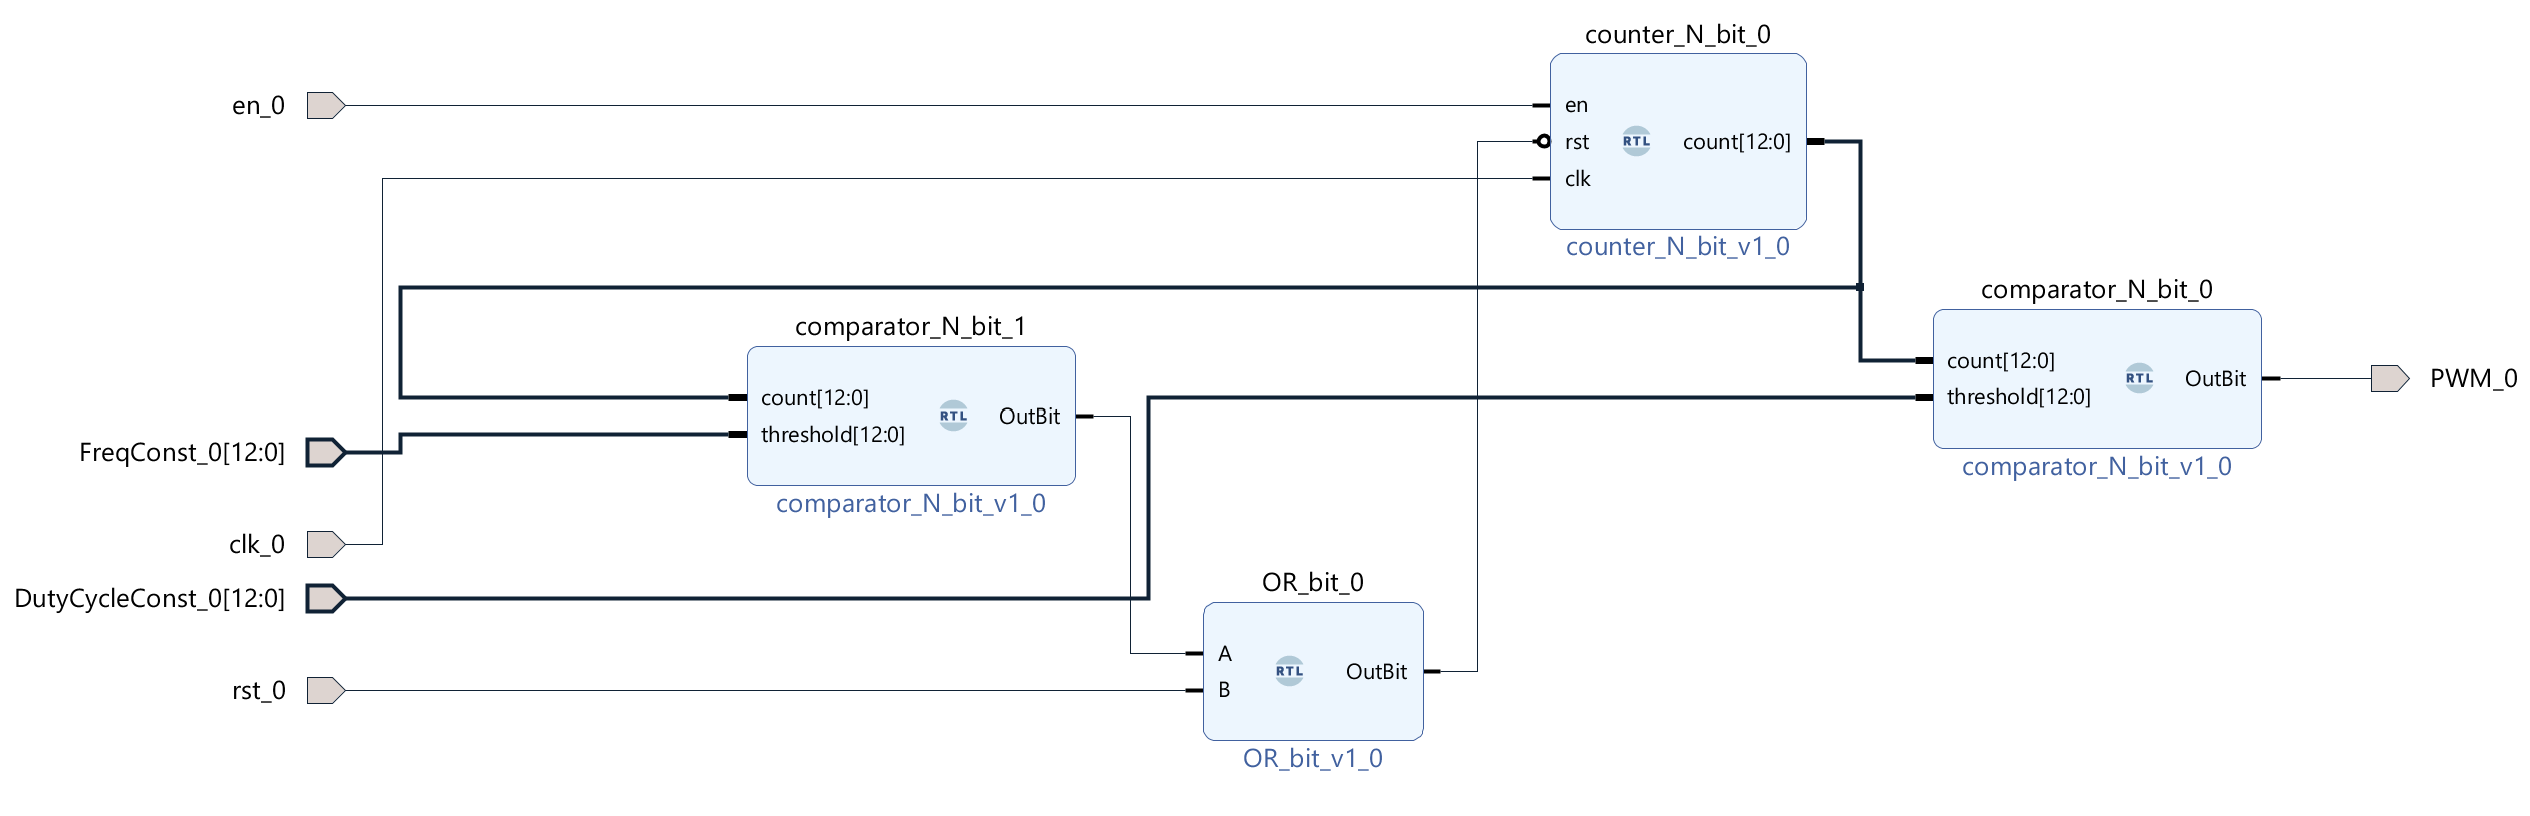
\includegraphics[width=1.2\textwidth]{figures/pwm/pwm_variable_block.png}}
    \caption{Block design of PWM module with variable pwm frequency and duty cycle.}
    \label{fig:pwm:block}
\end{figure}

The counter frequency is $f_{osc} = 100 [MHz]$ since it is connected to the clock driving the ZYNQ processing system implemented in the FPGA. The threshold for when to reset the counter can be calculated to achieve a frequency of $f_{PWM} = 20 [kHz]$.
\begin{equation}
    \frac{f_{osc}}{f_{PWM}} = 5000
\end{equation}
The amount of bits needed for the counter and comparators can now be calculated.
\begin{equation}
    Log_2(5000) = 12.29 \Rightarrow bits = 13
\end{equation}

\subsubsection{Simulating the PWM Module}
The PWM module is simulated with a duty cycle of $50 \%$ and the frequency is set to $20 [kHz]$. This is done by applying the calculated constants to the block design and tying the enable pin to '1' and reset pin to '0' as in \autoref{fig:pwm:block:connected}.

\begin{figure}[H]
    \centering
    \noindent\makebox[\textwidth][c]{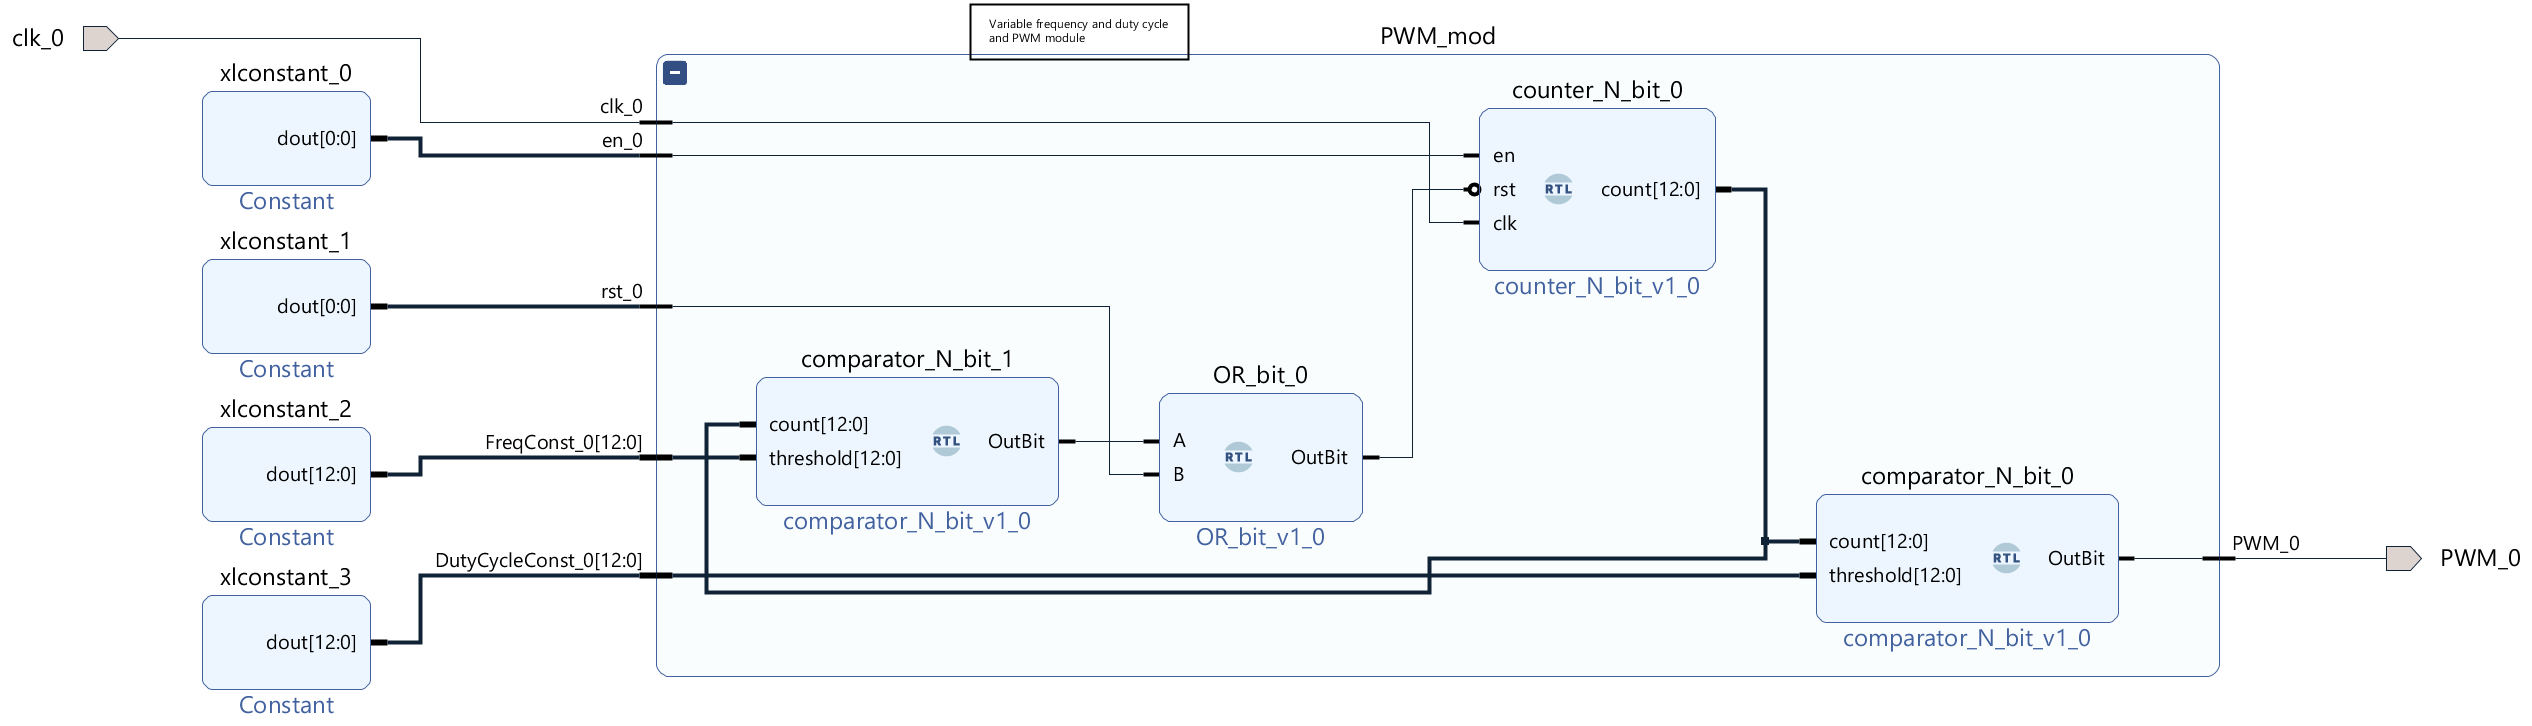
\includegraphics[width=1.2\textwidth]{figures/pwm/pwm_variable_block_heiarch.png}}
    \caption{A hierachy containing the PWM module is created and the constants is connected using VHDL constants.}
    \label{fig:pwm:block:connected}
\end{figure}

The simulation results are shown in \autoref{fig:pwm:simulation}.

\begin{figure}[H]
    \centering
    \noindent\makebox[\textwidth][c]{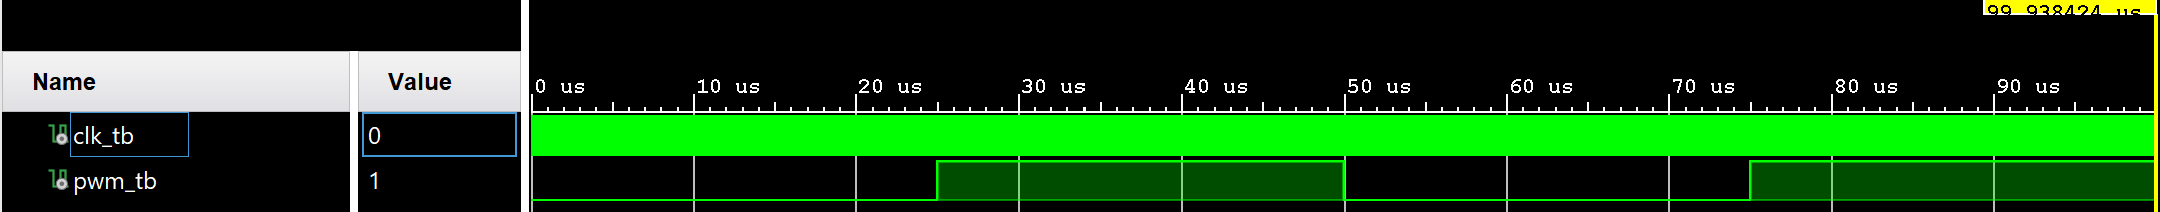
\includegraphics[width=1.2\textwidth]{figures/pwm/PWM_variable.png}}
    \caption{Test bench simulation of the designed variable PWM module.}
    \label{fig:pwm:simulation}
\end{figure}
It can be seen in \autoref{fig:pwm:simulation} that the PWM period is $T_{PWM} = 50 [\mu s]$, which confirms that a frequency of $\frac{1}{T_{PWM}} = f_{PWM} = 20 [kHz]$. Furthermore, the PWM switches between low and high at $t = 25 [\mu s]$, which gives yields a duty cycle of $50 \%$.

\subsection{Implementation of the Xilinx Analog to Digital Converter} \label{subsec:adc}
In this section, the analogue to digital converter on the Xilinx board, XADC, is set up by following the guide \cite{xadc_sdu}. The XADC is connected to the PS through an module in PL using Advanced eXtensible Interface, AXI; this is shown in figure \ref{fig:block_xadc}.

\begin{figure}[H]
    \centering    
    \noindent\makebox[\textwidth]{%
    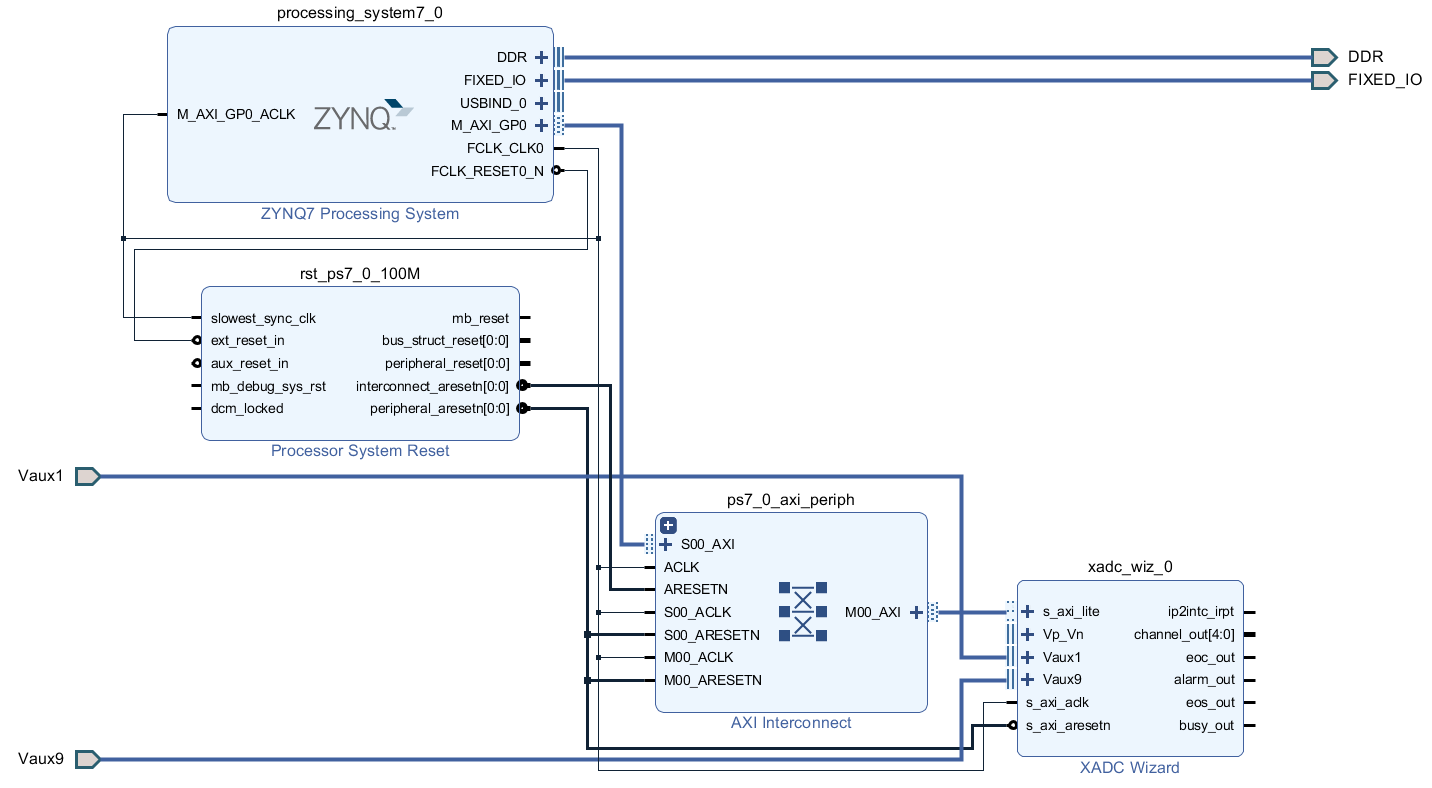
\includegraphics[width=1.2\textwidth]{figures/xadc/xadc.png}}
    \caption{Block design of XADC}
    \label{fig:block_xadc}
\end{figure}

The XADC is used to measure a voltage ranging from $[0, 3.3] V$, but the XADC can only accept voltage ranging between $[0, 1] V$. However, the pins $A0-A5$ on the PYNQ Z2 board scales down the input voltage from $3.3[V]$ to $1[V]$ via an internal voltage divider\cite{xadc_ref}, thus the pin $A0$ and pin $A1$ are used. In order to use the pins, it is necessary to state in the XADC wizard which Vaux ports that maps to I/O ports of the PYNQ Z2 board.  

\begin{figure}[H]
    \centering
    \begin{subfigure}[t]{0.49\textwidth}
        \centering
        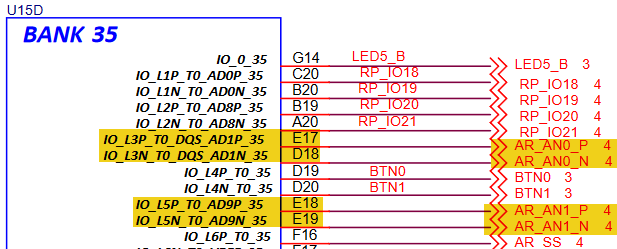
\includegraphics[width=0.9\textwidth]{figures/xadc/xadc_setup_pin_1.png}
        \captionsetup{width=0.9\textwidth}
        \caption{Schematic of I/O mapping of Arduino I/O}  
        \label{}
    \end{subfigure}
    \begin{subfigure}[t]{0.49\textwidth}  
        \centering 
        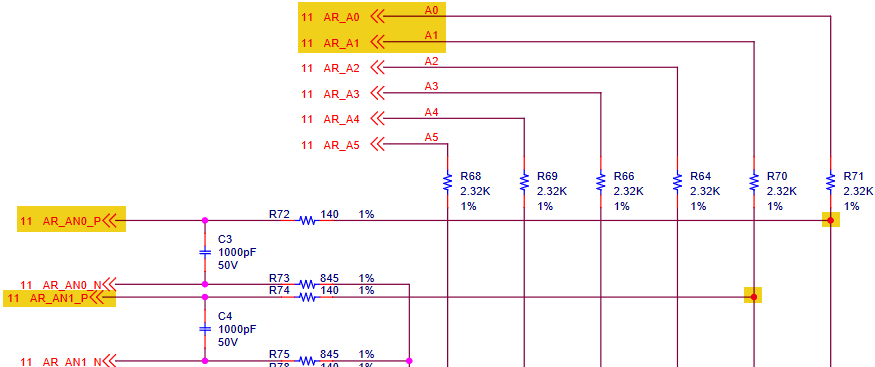
\includegraphics[width=0.9\textwidth]{figures/xadc/xadc_setup_pin_2.png}
        \captionsetup{width=0.9\textwidth}
        \caption{Schematic of bank 35}  
        \label{}
    \end{subfigure}
    \caption{PYNQ Z2 Schematic snip of bank 35 and I/O mapping of Arduino I/O\cite{pynq_z2_board_schematic}} 
    \label{fig:pynq_z2_schematic}
\end{figure}

From the schematic snippet of the PYNQ Z2 board illustrated in \autoref{fig:pynq_z2_schematic}, the pin $A0$'s positive and neutral maps to $D17$ and $D18$ respectively and pin $A1$'s positive and neutral maps to $E18$ and $E19$ respectively in bank 35. The bank values $
D17$ and $D18$ corresponds to Vaux1, and $E18$ and $E19$ corresponds to Vaux9 on the XADC wizard.

The XADC on the PYNQ Z2 board is a 12 bit ADC, which gives a resolution of $\frac{3.3[V]}{2^{12}} \approx 0.806 [mV]$ when meassuring voltages in range of $[0, 3.3] V$.

\subsubsection{Transfer PWM Value and Battery Percent to Block RAM}
% \begin{wrapfigure}{R}{0.4\textwidth}
%     \centering
%     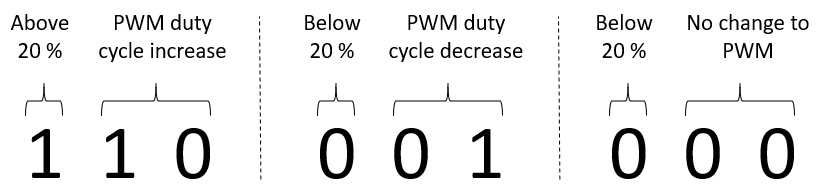
\includegraphics[width=0.2\textwidth]{figures/xadc/bitstream.png}
%     \captionsetup{width=0.35\textwidth}
%     \caption{Examples of the bitstream send to the PL.}
%     \label{fig:bitstream}
% \end{wrapfigure}
In order to regulate the battery charger circuit, a PS to PL communication were designed. The communication is done through a true dual-port block ram. The data send from the PS has a maximum size of 3 bits, and one address of the BRAM can hold 32 bits. Thus it is only necessary to write to one address. From the bitstream illustrated in \autoref{fig:bitstream}, it can be seen that the two bits contains the PWM duty cycle increase/decrease and the last bit contains whether the battery is above $20\%$ or not.

\begin{figure}[H]
    \centering
    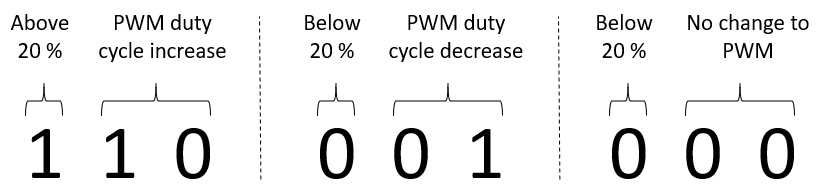
\includegraphics[width=0.75\textwidth]{figures/xadc/bitstream.png}
    \caption{Examples of the bitstream send to the PL.}
    \label{fig:bitstream}
\end{figure}

% In order to regulate the battery charger circuit a PS to PL communication were designed. The communication is done through true dual port block ram. The PWM increment or decrement value and battery percent values are together 4-bits in length, and a single address in the BRAM can hold up to 4 bytes, thus it is only necessary to write to one address. The first two-bits send to the BRAM contains the PWM-value and the next bits contains the battery percent value. 
The overall block diagram of the XADC and PS-PL communication is shown in \autoref{fig:block_xadc_ps_pl}.

\begin{figure}[H]
    \centering    
    \noindent\makebox[\textwidth]{%
    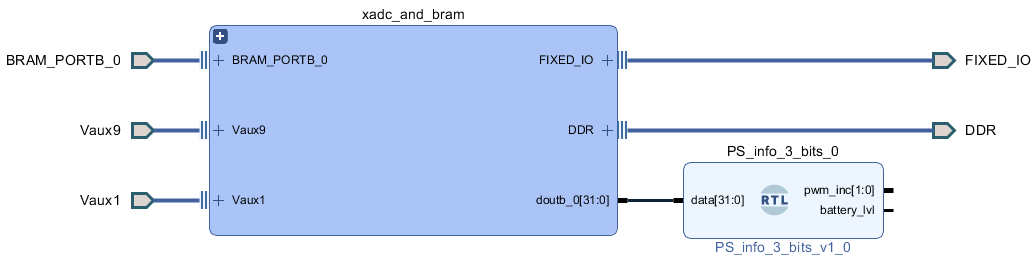
\includegraphics[width=1.2\textwidth]{figures/xadc/xadc_ps_pl_com.png}}
    \caption{Overall block design of XADC and PS-PL communication}
    \label{fig:block_xadc_ps_pl}
\end{figure}

The overall block design consist of two modules. The module \texttt{PS\_info\_3\_bits\_0} splits the data read from the BRAM into the PWM-value and battery percentage value. The hierarchy module \texttt{xadc\_and\_bram} takes care of the XADC and PS to PL communication which is illustrated in \autoref{fig:block_xadc_ps_pl_inside}. 

\begin{figure}[H]
    \centering    
    \noindent\makebox[\textwidth]{%
    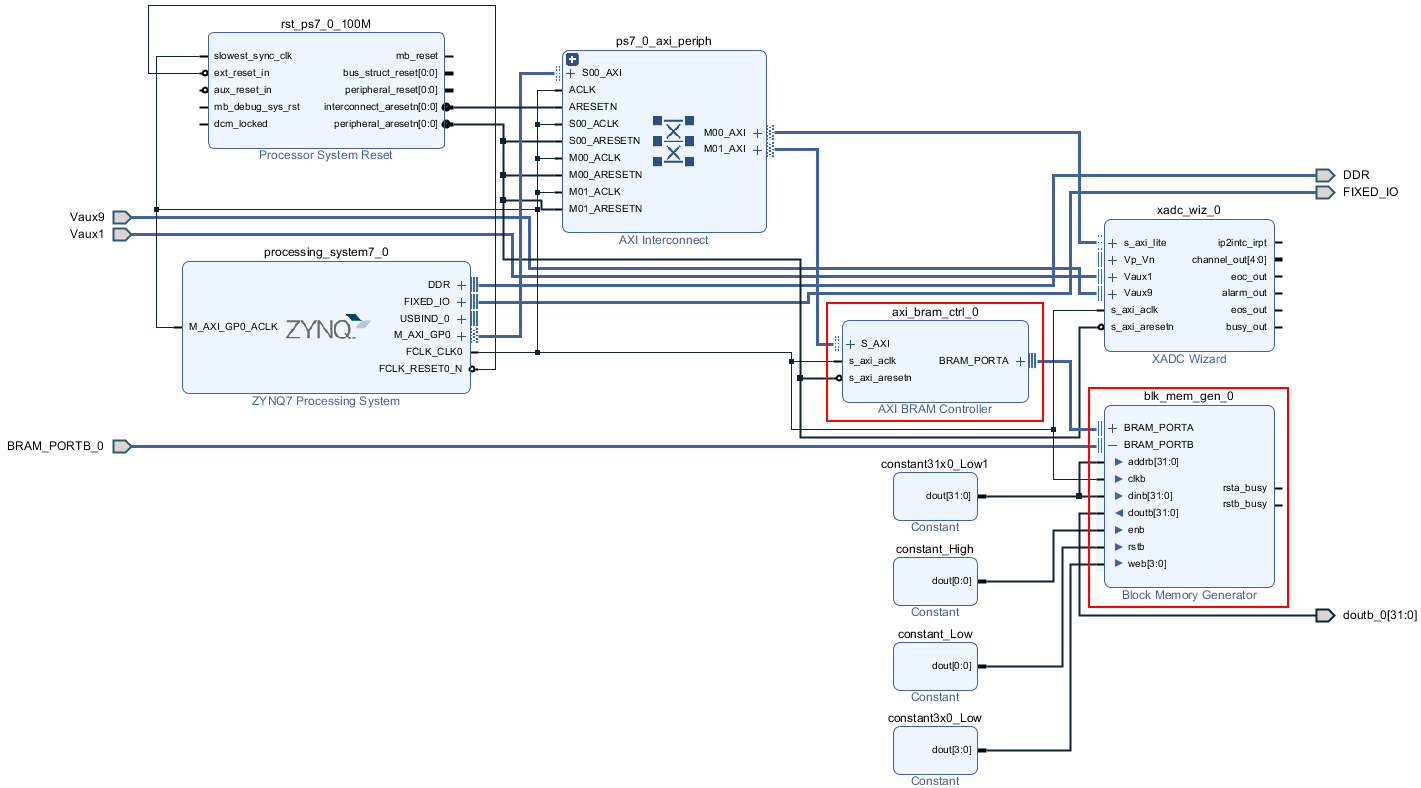
\includegraphics[width=1.2\textwidth]{figures/xadc/xadc_ps_pl_com_inside.png}}
    \caption{Block design of hierarchy module \texttt{xadc\_and\_bram}.}
    \label{fig:block_xadc_ps_pl_inside}
\end{figure}

The block design in \autoref{fig:block_xadc_ps_pl_inside} has the same main element as the block design of the XADC shown in \autoref{fig:block_xadc}. The two major components added in contrast to the XADC block design are an AXI BRAM Controller and a Block Memory Generator which are marked with red. 

\textbf{Testing the XADC}\\
A physical test was conducted to confirm both the XADC and the PS to PL communication worked as intended. This was done by measuring a voltage ranging of $[0, 3] V$ on the PYNQ™ Z2 board's $A1$ pin and writing the value to the BRAM. The FPGA then reads the value and shows it on a Vishay TDSR1360 7-segment display. The block design used to conduct the test is shown in \autoref{fig:block_xadc_bram_7seg}.

\begin{figure}[H]
    \centering    
    \noindent\makebox[\textwidth]{%
    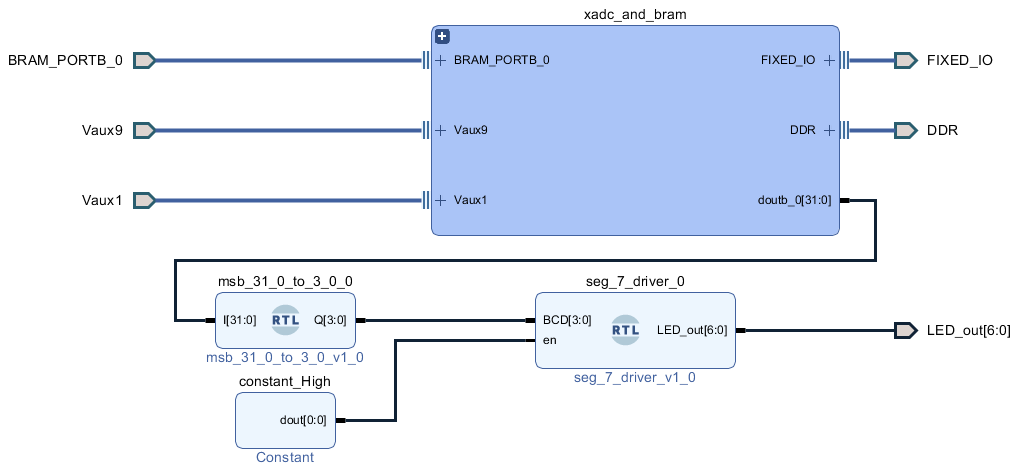
\includegraphics[width=1.2\textwidth]{figures/xadc/xadc_bram_7seg.png}}
    \caption{Block design used when testing XADC and PS to PL communication.}
    \label{fig:block_xadc_bram_7seg}
\end{figure}

The results from the test can be seen in \autoref{fig:adx_bram_7seg_results}.

\begin{figure}[H]
    \centering
    \begin{subfigure}[t]{0.45\textwidth}
        \centering
        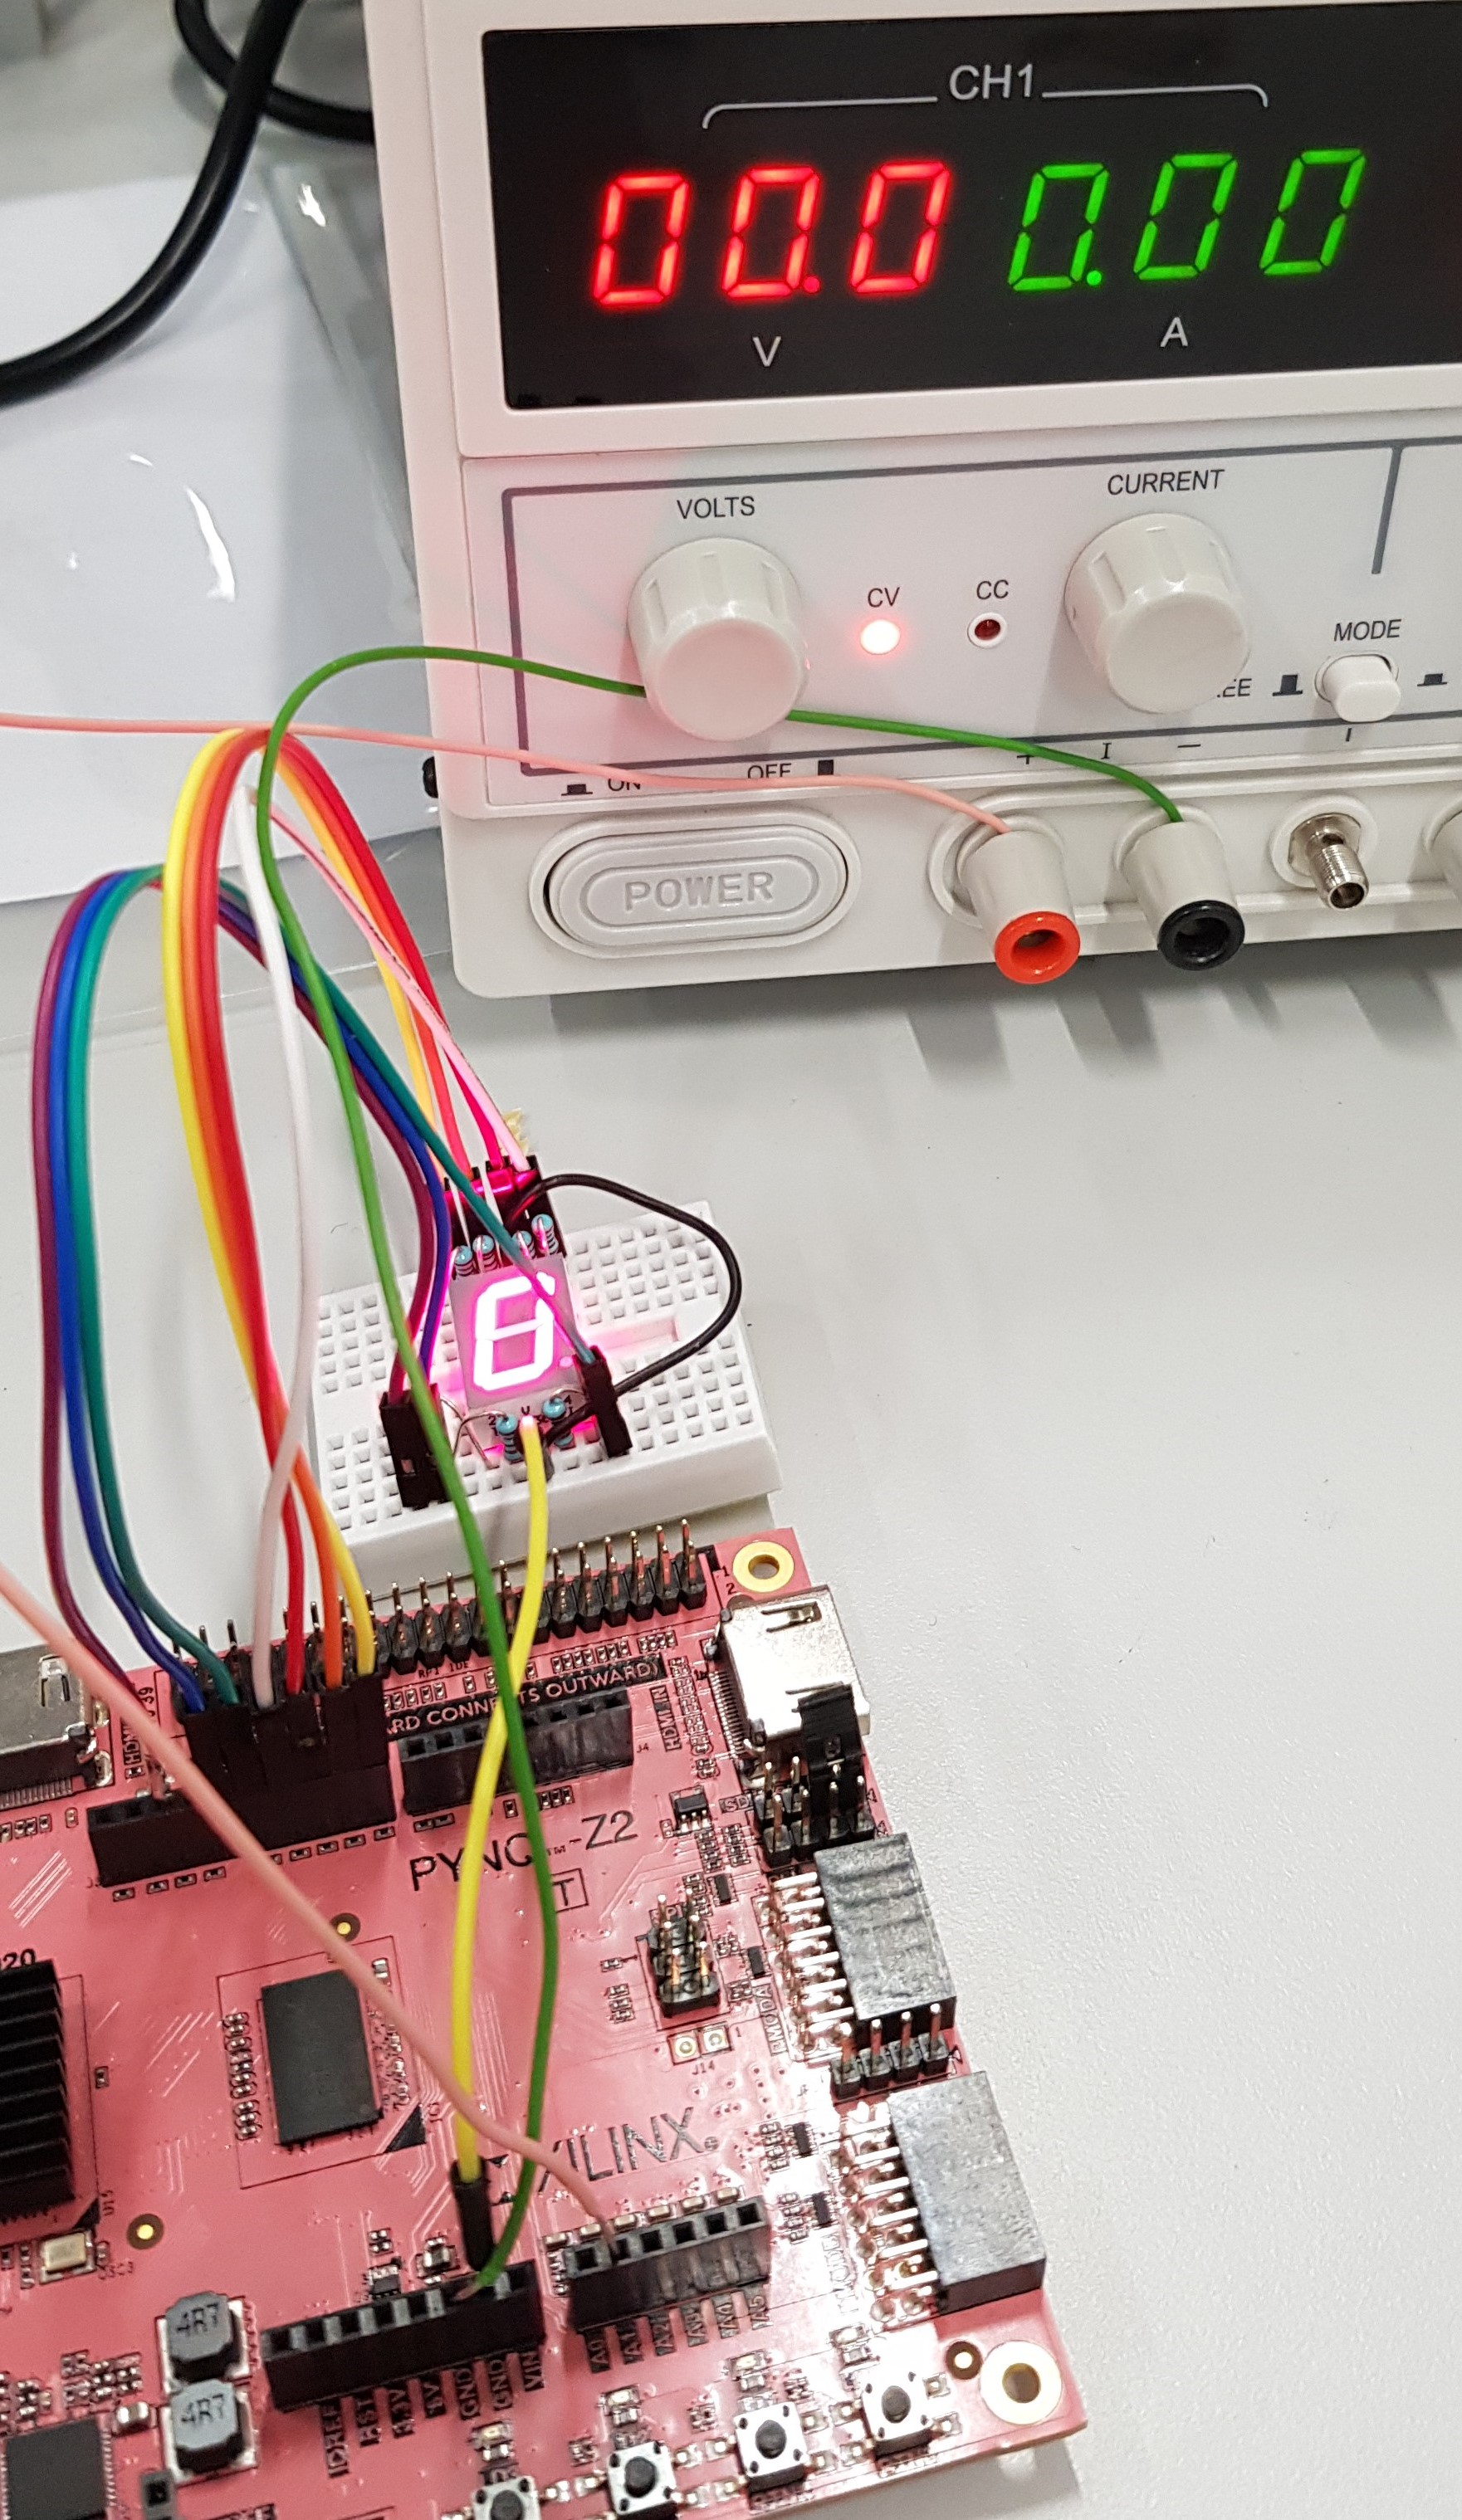
\includegraphics[width=0.8\textwidth]{figures/xadc/0V_result.jpg}
        \captionsetup{width=0.8\textwidth}
        \caption{0 [V] measured by the ADC displays 0 on the 7-segment display.}  
        \label{}
    \end{subfigure}
    \begin{subfigure}[t]{0.45\textwidth}  
        \centering 
        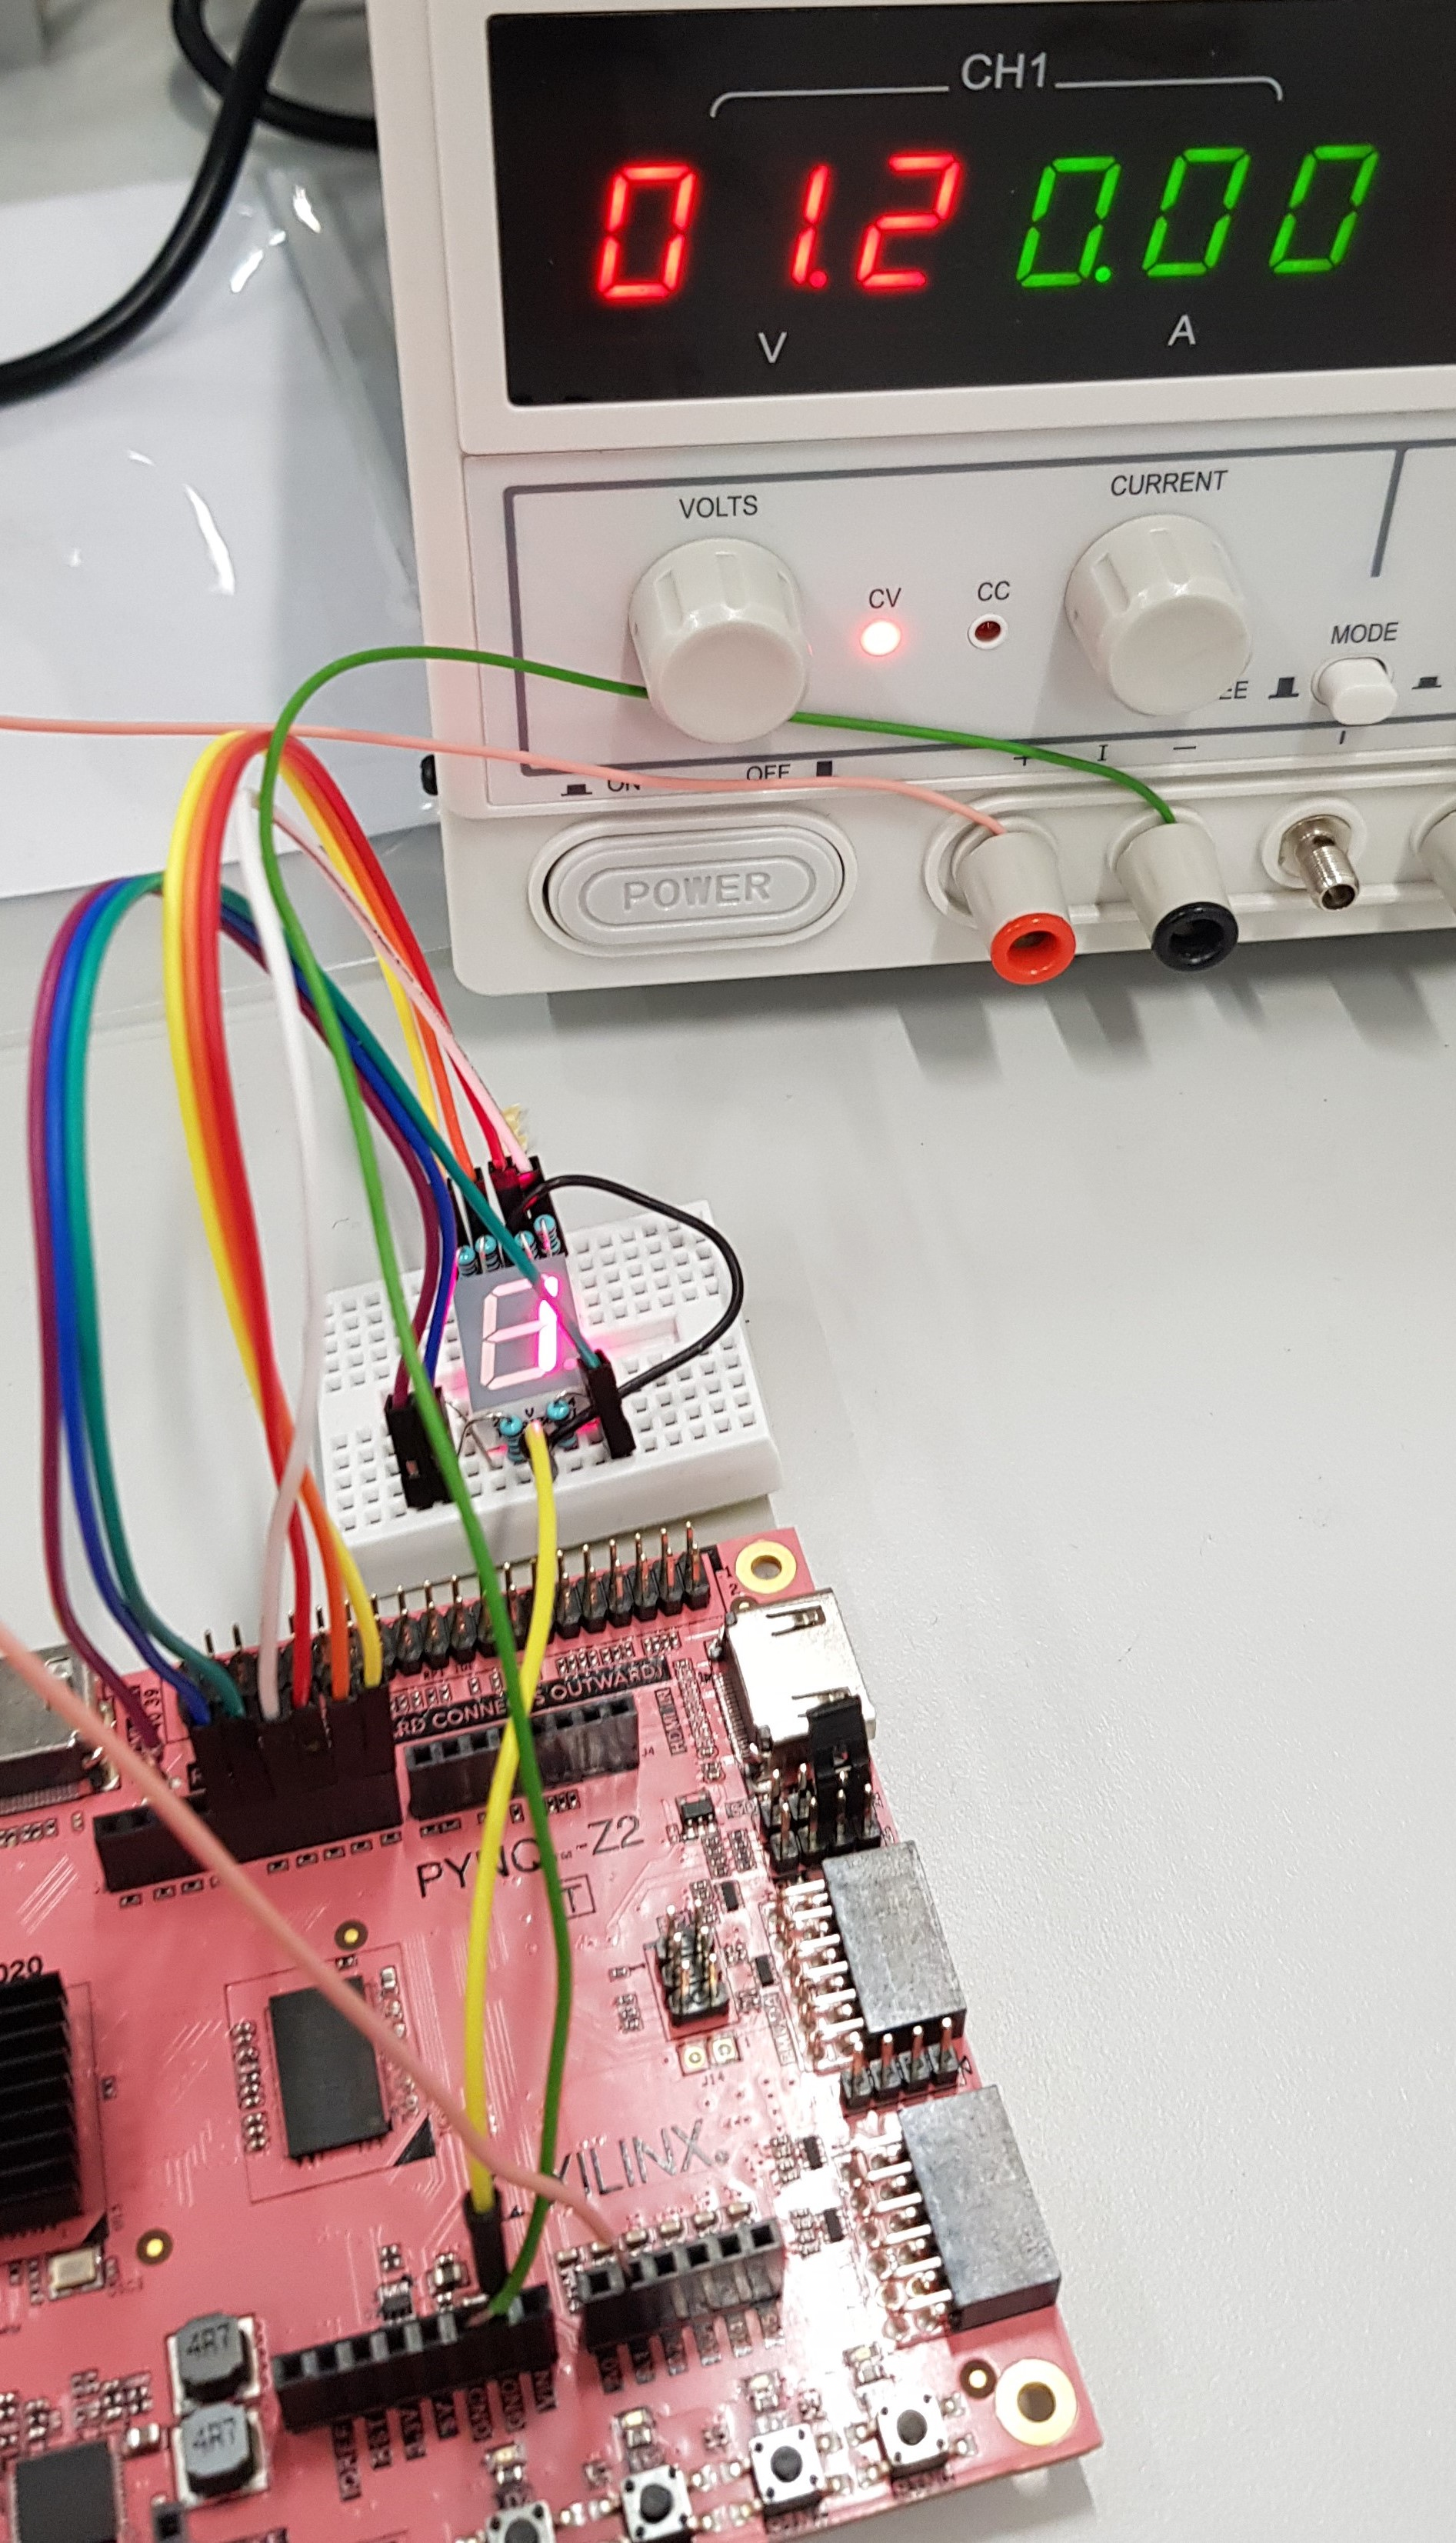
\includegraphics[width=0.8\textwidth]{figures/xadc/1V_result.jpg}
        \captionsetup{width=0.8\textwidth}
        \caption{1.2 [V] measured by the ADC displays 1 on the 7-segment display.}  
        \label{}
    \end{subfigure}
    
    \begin{subfigure}[t]{0.45\textwidth}   
        \centering 
        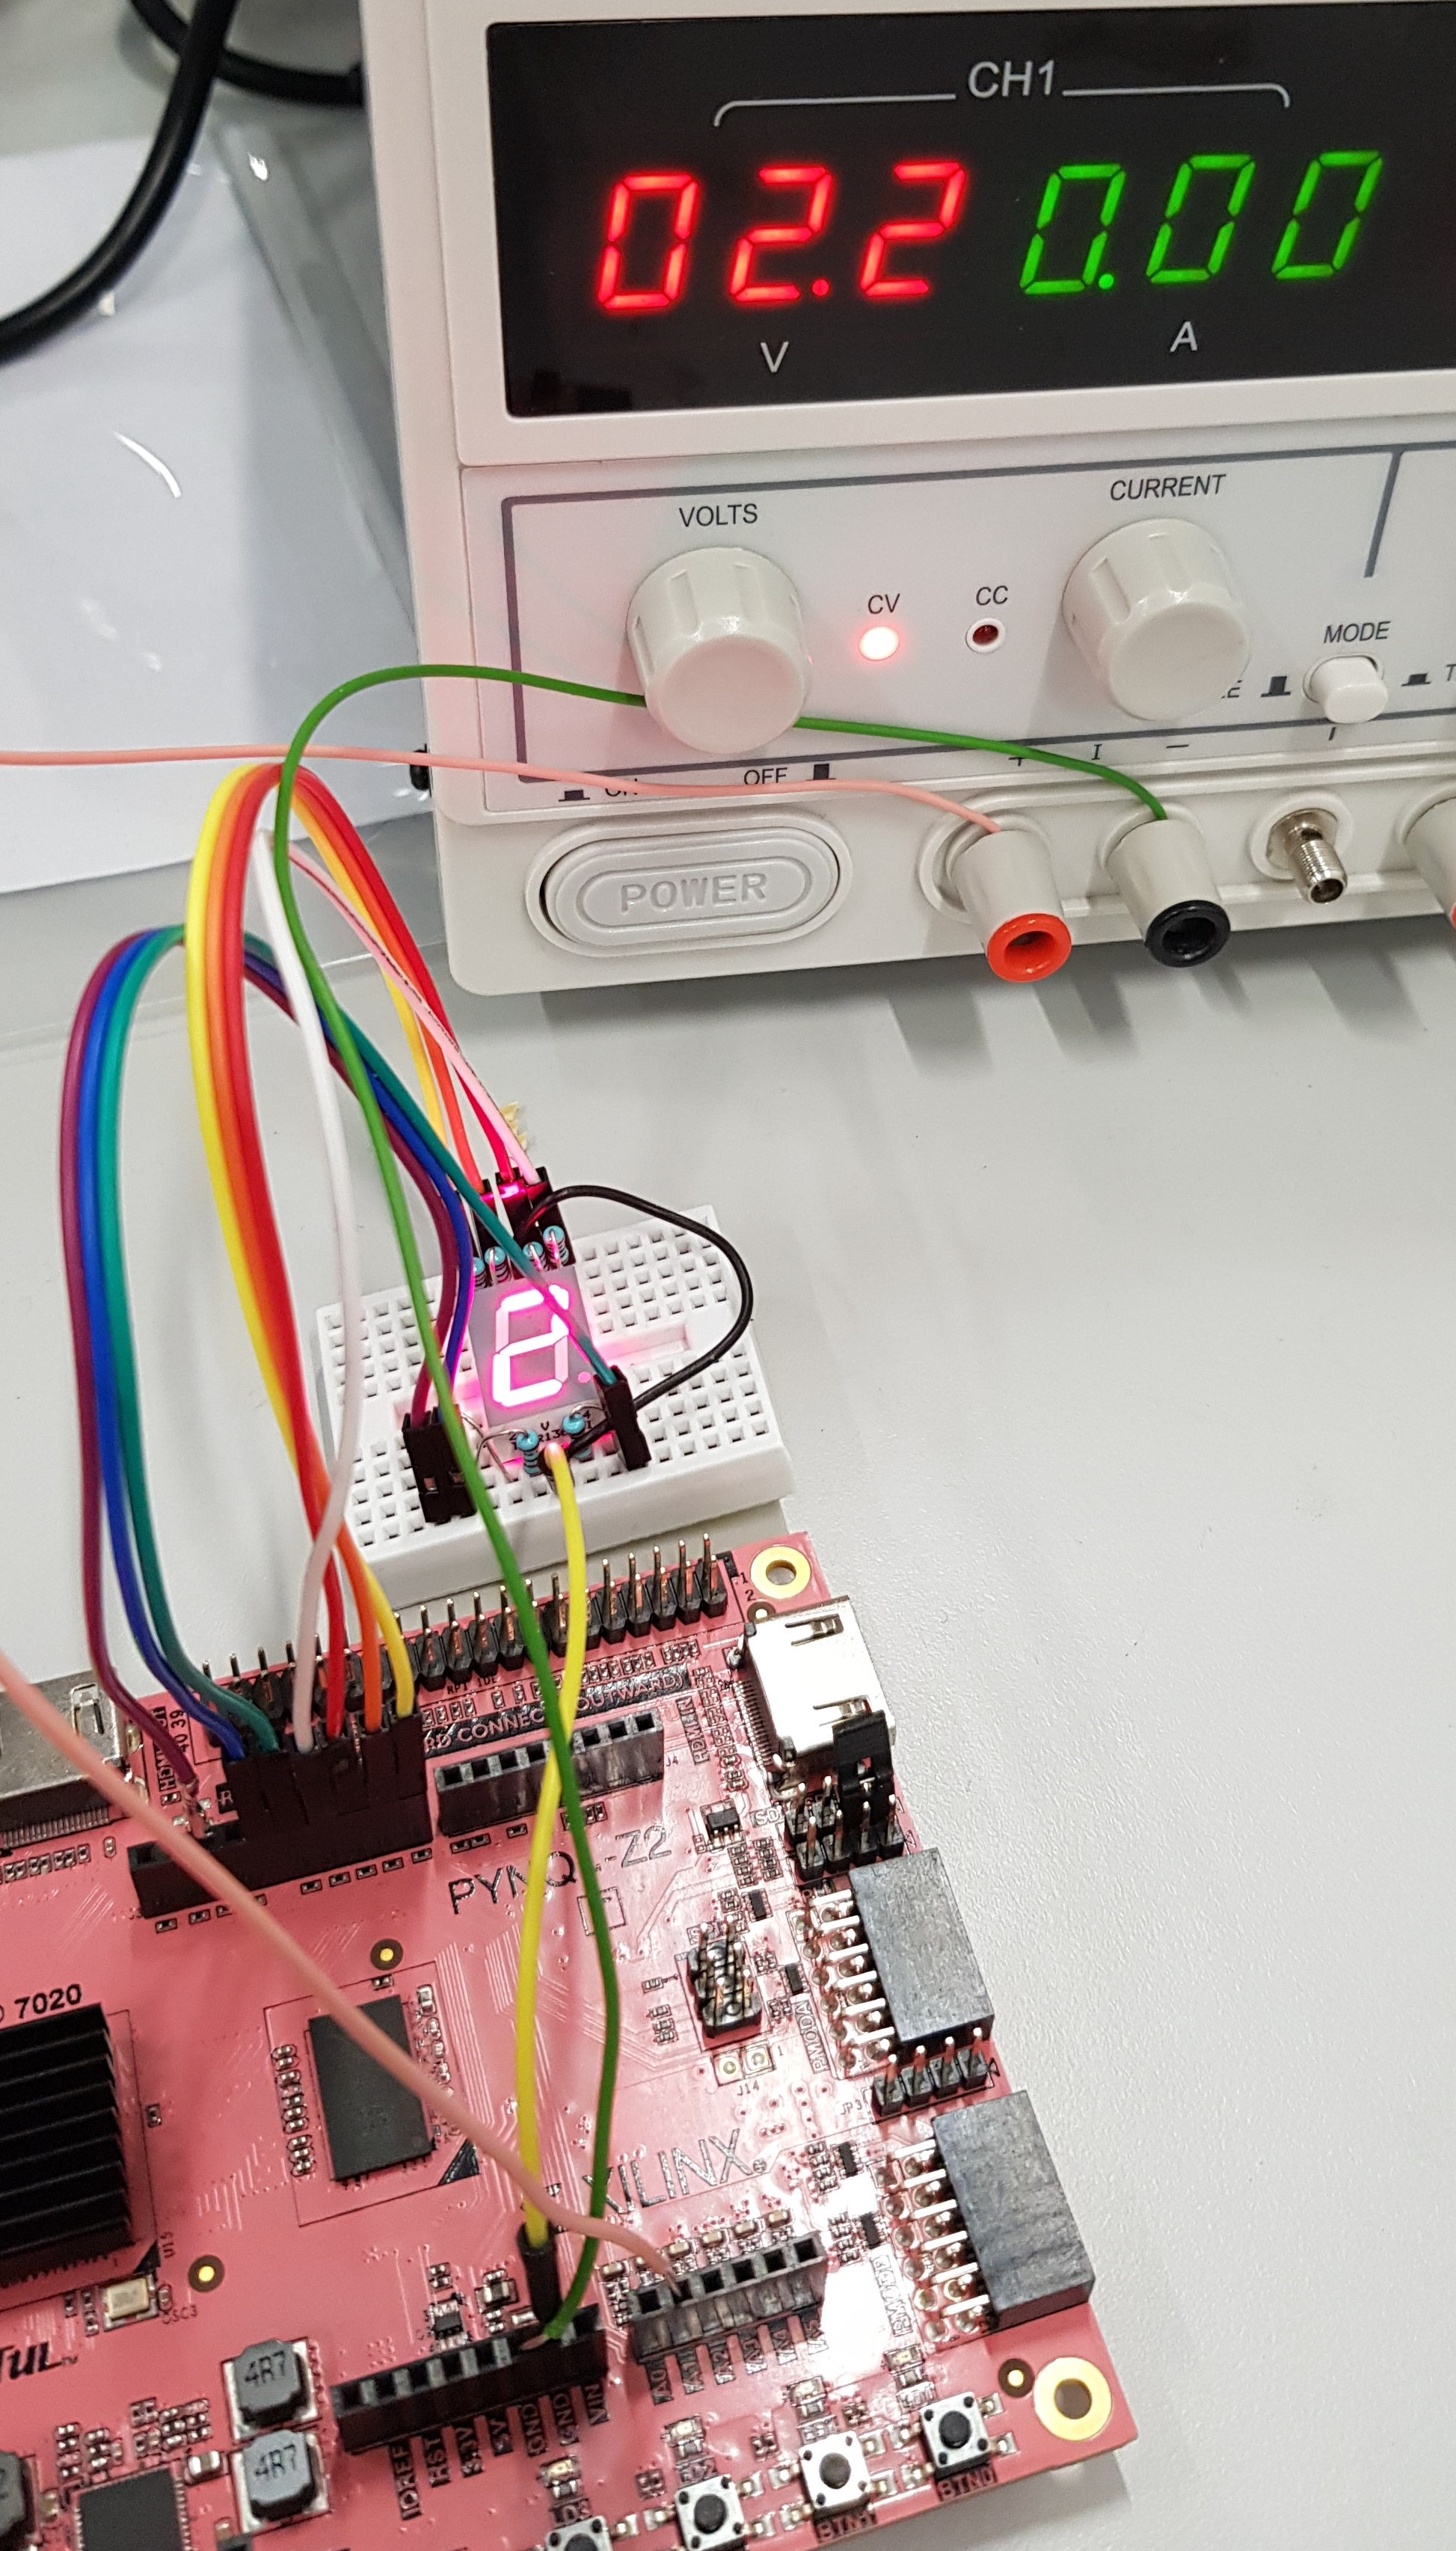
\includegraphics[width=0.8\textwidth]{figures/xadc/2V_result.jpg}
        \captionsetup{width=0.8\textwidth}
        \caption{2.2 [V] measured by the ADC displays 2 on the 7-segment display.}  
        \label{}
    \end{subfigure}
    \begin{subfigure}[t]{0.45\textwidth}   
        \centering 
        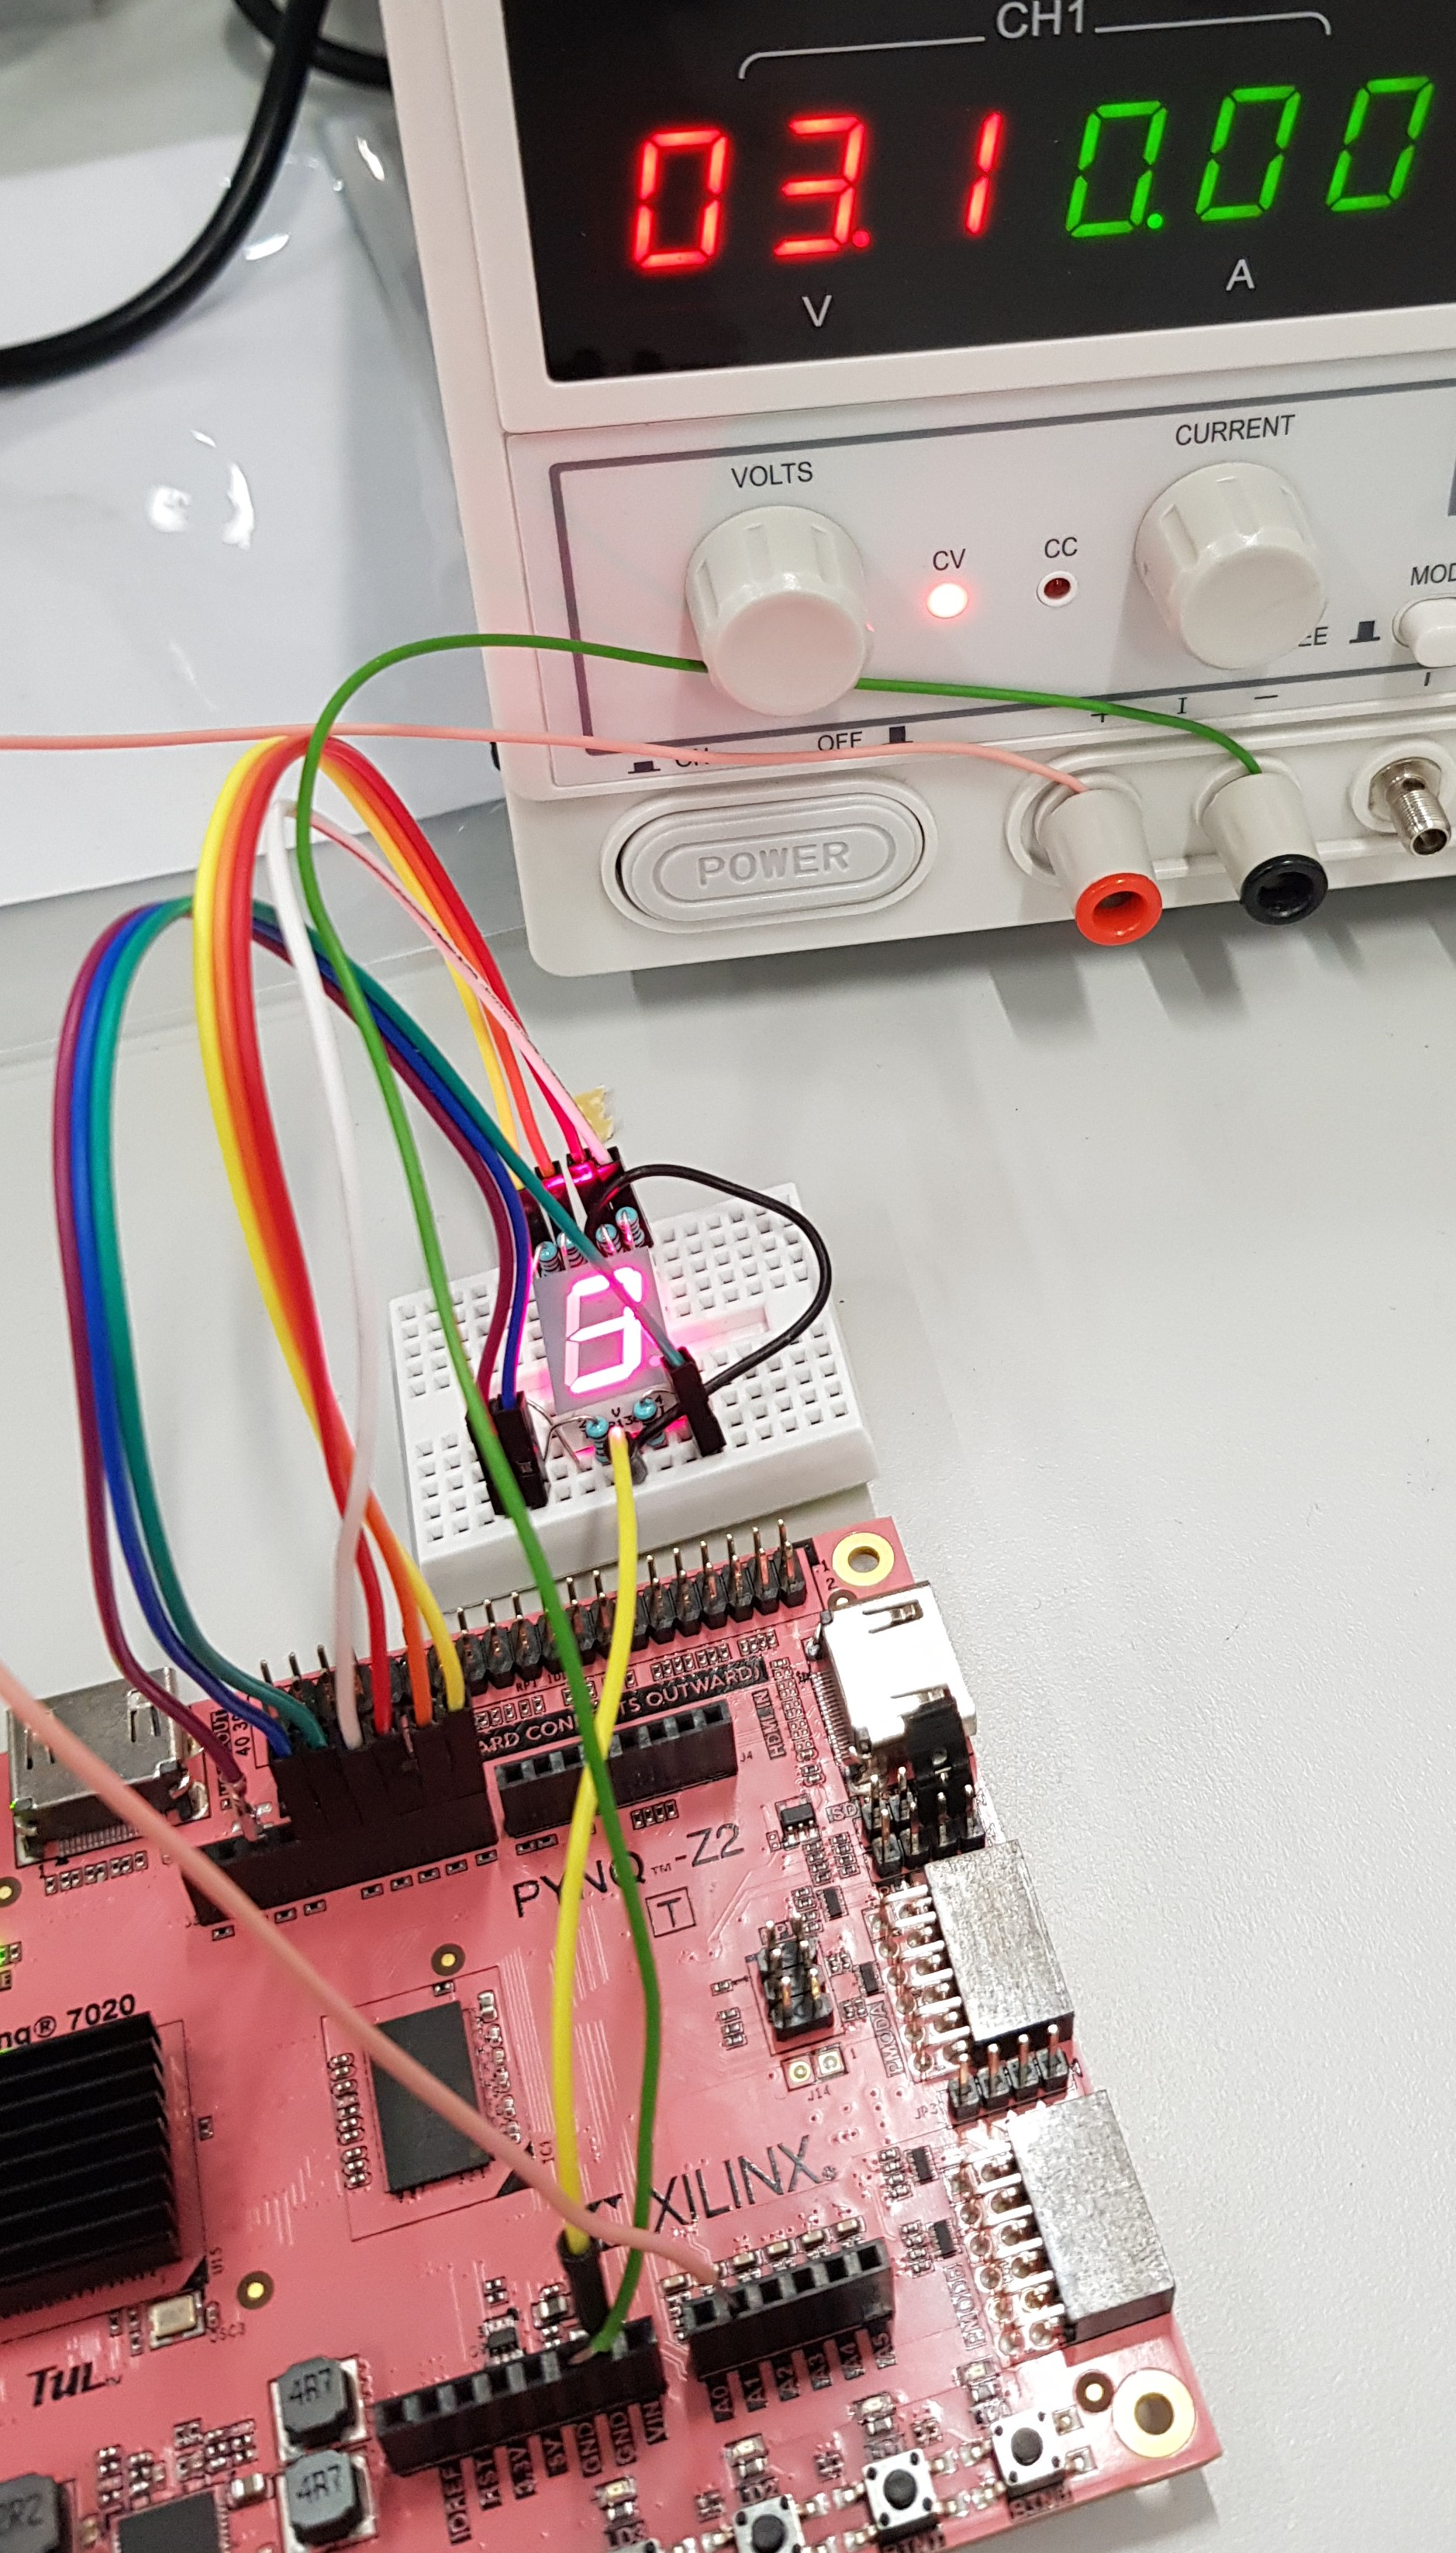
\includegraphics[width=0.8\textwidth]{figures/xadc/3V_result.jpg}
        \captionsetup{width=0.8\textwidth}
        \caption{3.1 [V] measured by the ADC displays 3 on the 7-segment display.}     
        \label{}
    \end{subfigure}
    \caption{Test results of measured voltage with XADC using PS to PL communication to show value on bcd display} 
    \label{fig:adx_bram_7seg_results}
\end{figure}

From the results in \autoref{fig:adx_bram_7seg_results} it can be concluded the integer of the voltage measured via the XADC is being transferred to the FPGA via PS to PL communication.

\end{document}